\documentclass[conference]{IEEEtran}
% *** MISC UTILITY PACKAGES ***
%\usepackage{ifpdf}
% Heiko Oberdiek's ifpdf.sty is very useful if you need conditional
% compilation based on whether the output is pdf or dvi.
% usage:
% \ifpdf
%   % pdf code
% \else
%   % dvi code
% \fi
% The latest version of ifpdf.sty can be obtained from:
% http://www.ctan.org/pkg/ifpdf
% Also, note that IEEEtran.cls V1.7 and later provides a builtin
% \ifCLASSINFOpdf conditional that works the same way.
% When switching from latex to pdflatex and vice-versa, the compiler may
% have to be run twice to clear warning/error messages.

% *** GRAPHICS RELATED PACKAGES ***
\ifCLASSINFOpdf
   \usepackage[pdftex]{graphicx}
  % declare the path(s) where your graphic files are
   \graphicspath{{../pdf/}{../jpeg/}}
  % and their extensions so you won't have to specify these with
  % every instance of \includegraphics
   \DeclareGraphicsExtensions{.pdf,.jpeg,.png}
\else
  % or other class option (dvipsone, dvipdf, if not using dvips). graphicx
  % will default to the driver specified in the system graphics.cfg if no
  % driver is specified.
   \usepackage[dvips]{graphicx}
  % declare the path(s) where your graphic files are
   \graphicspath{{../eps/}}
  % and their extensions so you won't have to specify these with
  % every instance of \includegraphics
   \DeclareGraphicsExtensions{.eps}
\fi
% graphicx was written by David Carlisle and Sebastian Rahtz. It is
% required if you want graphics, photos, etc. graphicx.sty is already
% installed on most LaTeX systems. The latest version and documentation
% can be obtained at:
% http://www.ctan.org/pkg/graphicx
% Another good source of documentation is "Using Imported Graphics in
% LaTeX2e" by Keith Reckdahl which can be found at:
% http://www.ctan.org/pkg/epslatex
%
% latex, and pdflatex in dvi mode, support graphics in encapsulated
% postscript (.eps) format. pdflatex in pdf mode supports graphics
% in .pdf, .jpeg, .png and .mps (metapost) formats. Users should ensure
% that all non-photo figures use a vector format (.eps, .pdf, .mps) and
% not a bitmapped formats (.jpeg, .png). The IEEE frowns on bitmapped formats
% which can result in "jaggedy"/blurry rendering of lines and letters as
% well as large increases in file sizes.
%
% You can find documentation about the pdfTeX application at:
% http://www.tug.org/applications/pdftex

% *** MATH PACKAGES ***
%
%\usepackage{amsmath}
% A popular package from the American Mathematical Society that provides
% many useful and powerful commands for dealing with mathematics.
%
% Note that the amsmath package sets \interdisplaylinepenalty to 10000
% thus preventing page breaks from occurring within multiline equations. Use:
%\interdisplaylinepenalty=2500
% after loading amsmath to restore such page breaks as IEEEtran.cls normally
% does. amsmath.sty is already installed on most LaTeX systems. The latest
% version and documentation can be obtained at:
% http://www.ctan.org/pkg/amsmath

% *** ALIGNMENT PACKAGES ***
%
%\usepackage{array}
% Frank Mittelbach's and David Carlisle's array.sty patches and improves
% the standard LaTeX2e array and tabular environments to provide better
% appearance and additional user controls. As the default LaTeX2e table
% generation code is lacking to the point of almost being broken with
% respect to the quality of the end results, all users are strongly
% advised to use an enhanced (at the very least that provided by array.sty)
% set of table tools. array.sty is already installed on most systems. The
% latest version and documentation can be obtained at:
% http://www.ctan.org/pkg/array


% IEEEtran contains the IEEEeqnarray family of commands that can be used to
% generate multiline equations as well as matrices, tables, etc., of high
% quality.

% *** SUBFIGURE PACKAGES ***
\ifCLASSOPTIONcompsoc
  \usepackage[caption=false,font=normalsize,labelfont=sf,textfont=sf]{subfig}
\else
  \usepackage[caption=false,font=footnotesize]{subfig}
\fi
% subfig.sty, written by Steven Douglas Cochran, is the modern replacement
% for subfigure.sty, the latter of which is no longer maintained and is
% incompatible with some LaTeX packages including fixltx2e. However,
% subfig.sty requires and automatically loads Axel Sommerfeldt's caption.sty
% which will override IEEEtran.cls' handling of captions and this will result
% in non-IEEE style figure/table captions. To prevent this problem, be sure
% and invoke subfig.sty's "caption=false" package option (available since
% subfig.sty version 1.3, 2005/06/28) as this is will preserve IEEEtran.cls
% handling of captions.
% Note that the Computer Society format requires a larger sans serif font
% than the serif footnote size font used in traditional IEEE formatting
% and thus the need to invoke different subfig.sty package options depending
% on whether compsoc mode has been enabled.
%
% The latest version and documentation of subfig.sty can be obtained at:
% http://www.ctan.org/pkg/subfig

% *** FLOAT PACKAGES ***
%
%\usepackage{fixltx2e}
% fixltx2e, the successor to the earlier fix2col.sty, was written by
% Frank Mittelbach and David Carlisle. This package corrects a few problems
% in the LaTeX2e kernel, the most notable of which is that in current
% LaTeX2e releases, the ordering of single and double column floats is not
% guaranteed to be preserved. Thus, an unpatched LaTeX2e can allow a
% single column figure to be placed prior to an earlier double column
% figure.
% Be aware that LaTeX2e kernels dated 2015 and later have fixltx2e.sty's
% corrections already built into the system in which case a warning will
% be issued if an attempt is made to load fixltx2e.sty as it is no longer
% needed.
% The latest version and documentation can be found at:
% http://www.ctan.org/pkg/fixltx2e

%\usepackage{stfloats}
% stfloats.sty was written by Sigitas Tolusis. This package gives LaTeX2e
% the ability to do double column floats at the bottom of the page as well
% as the top. (e.g., "\begin{figure*}[!b]" is not normally possible in
% LaTeX2e). It also provides a command:
%\fnbelowfloat
% to enable the placement of footnotes below bottom floats (the standard
% LaTeX2e kernel puts them above bottom floats). This is an invasive package
% which rewrites many portions of the LaTeX2e float routines. It may not work
% with other packages that modify the LaTeX2e float routines. The latest
% version and documentation can be obtained at:
% http://www.ctan.org/pkg/stfloats
% Do not use the stfloats baselinefloat ability as the IEEE does not allow
% \baselineskip to stretch. Authors submitting work to the IEEE should note
% that the IEEE rarely uses double column equations and that authors should try
% to avoid such use. Do not be tempted to use the cuted.sty or midfloat.sty
% packages (also by Sigitas Tolusis) as the IEEE does not format its papers in
% such ways.
% Do not attempt to use stfloats with fixltx2e as they are incompatible.
% Instead, use Morten Hogholm'a dblfloatfix which combines the features
% of both fixltx2e and stfloats:
% \usepackage{dblfloatfix}
% The latest version can be found at:
% http://www.ctan.org/pkg/dblfloatfix

% *** PDF, URL AND HYPERLINK PACKAGES ***
%
\usepackage{url}
\usepackage{tabu}
% url.sty was written by Donald Arseneau. It provides better support for
% handling and breaking URLs. url.sty is already installed on most LaTeX
% systems. The latest version and documentation can be obtained at:
% http://www.ctan.org/pkg/url
% Basically, \url{my_url_here}.

% *** Do not adjust lengths that control margins, column widths, etc. ***
% *** Do not use packages that alter fonts (such as pslatex).         ***
% There should be no need to do such things with IEEEtran.cls V1.6 and later.
% (Unless specifically asked to do so by the journal or conference you plan
% to submit to, of course. )

% An example of a floating figure using the graphicx package.
% Note that \label must occur AFTER (or within) \caption.
% For figures, \caption should occur after the \includegraphics.
% Note that IEEEtran v1.7 and later has special internal code that
% is designed to preserve the operation of \label within \caption
% even when the captionsoff option is in effect. However, because
% of issues like this, it may be the safest practice to put all your
% \label just after \caption rather than within \caption{}.
%
% Reminder: the "draftcls" or "draftclsnofoot", not "draft", class
% option should be used if it is desired that the figures are to be
% displayed while in draft mode.
%

% Note that the IEEE typically puts floats only at the top, even when this
% results in a large percentage of a column being occupied by floats.

% An example of a double column floating figure using two subfigures.
% (The subfig.sty package must be loaded for this to work.)
% The subfigure \label commands are set within each subfloat command,
% and the \label for the overall figure must come after \caption.
% \hfil is used as a separator to get equal spacing.
% Watch out that the combined width of all the subfigures on a
% line do not exceed the text width or a line break will occur.
%
%\begin{figure*}[!t]
%\centering
%\subfloat[Case I]{\includegraphics[width=2.5in]{box}%
%\label{fig_first_case}}
%\hfil
%\subfloat[Case II]{\includegraphics[width=2.5in]{box}%
%\label{fig_second_case}}
%\caption{Simulation results for the network.}
%\label{fig_sim}
%\end{figure*}
%
% Note that often IEEE papers with subfigures do not employ subfigure
% captions (using the optional argument to \subfloat[]), but instead will
% reference/describe all of them (a), (b), etc., within the main caption.
% Be aware that for subfig.sty to generate the (a), (b), etc., subfigure
% labels, the optional argument to \subfloat must be present. If a
% subcaption is not desired, just leave its contents blank,
% e.g., \subfloat[].

% An example of a floating table. Note that, for IEEE style tables, the
% \caption command should come BEFORE the table and, given that table
% captions serve much like titles, are usually capitalized except for words
% such as a, an, and, as, at, but, by, for, in, nor, of, on, or, the, to
% and up, which are usually not capitalized unless they are the first or
% last word of the caption. Table text will default to \footnotesize as
% the IEEE normally uses this smaller font for tables.
% The \label must come after \caption as always.
%
%\begin{table}[!t]
%% increase table row spacing, adjust to taste
%\renewcommand{\arraystretch}{1.3}
% if using array.sty, it might be a good idea to tweak the value of
% \extrarowheight as needed to properly center the text within the cells
%\caption{An Example of a Table}
%\label{table_example}
%\centering
%% Some packages, such as MDW tools, offer better commands for making tables
%% than the plain LaTeX2e tabular which is used here.
%\begin{tabular}{|c||c|}
%\hline
%One & Two\\
%\hline
%Three & Four\\
%\hline
%\end{tabular}
%\end{table}

% Note that the IEEE does not put floats in the very first column
% - or typically anywhere on the first page for that matter. Also,
% in-text middle ("here") positioning is typically not used, but it
% is allowed and encouraged for Computer Society conferences (but
% not Computer Society journals). Most IEEE journals/conferences use
% top floats exclusively.
% Note that, LaTeX2e, unlike IEEE journals/conferences, places
% footnotes above bottom floats. This can be corrected via the
% \fnbelowfloat command of the stfloats package.

% For peer review papers, you can put extra information on the cover
% page as needed:
% \ifCLASSOPTIONpeerreview
% \begin{center} \bfseries EDICS Category: 3-BBND \end{center}
% \fi
%
% For peerreview papers, this IEEEtran command inserts a page break and
% creates the second title. It will be ignored for other modes.

% correct bad hyphenation here
\hyphenation{op-tical net-works semi-conduc-tor}

\begin{document}
\title{Emerging Threats and Defenses Regarding Denial of Service in the Network and Transport Layers}

% author names and affiliations
\author{\IEEEauthorblockN{Darius Saif}
\IEEEauthorblockA{Carleton University\\
Darius.Saif@Carleton.ca}
\and
\IEEEauthorblockN{Alexandre Cormier}
\IEEEauthorblockA{Carleton University\\
Alexandre.Cormier@Carleton.ca}
\and
\IEEEauthorblockN{Suranjit Banik}
\IEEEauthorblockA{University of Ottawa\\
Sbani041@UOttawa.ca}}

% make the title area
\maketitle

\begin{abstract}
%Refresh this?
Denial of Service (DoS), and their larger-scale variant Distributed Denial of Service (DDoS), attacks seek out and exploit various network vulnerabilities in order to overwhelm a node to the point of severe impairment. This may lead to outages for legitimate clients making requests to servers and can also gravely affect peer-to-peer infrastructures. These attacks prey on protocols residing in numerous layers of the Open Systems Interconnection (OSI) model and fall under different sub-categories. Well-known attacks in this field are SYN flooding, Teardrop, Local Area Network Denial (LAND), as well as both User Datagram Protocol (UDP) and Internet Control Message Protocol (ICMP) flooding. As the number of users and services accommodated by the Internet increases, many emerging technologies exist to further improve network performance. With innovative notions such as Software Defined Networking (SDN) and cloud computing, taking precautions against DoS-based attacks is of the utmost importance. This survey aims to address the latest strides in both attack methodologies and defense mechanisms specific to the network and transport layers of the OSI model.
\end{abstract}

\begin{IEEEkeywords}
Survey,
Denial of Service,
Reflective Attack,
LDoS,
DDoS Defense,
Network Layer,
Transport Layer,
Cloud Computing,
Software Defined Networking,
Botnets
\end{IEEEkeywords}
% no keywords

\IEEEpeerreviewmaketitle

\section{Introduction}
Denial of Service (DoS) is a class of networking attacks which, as the name suggests, seek to bring a particular node, resource, or application down for a period of time --- denying potential users of accessing such a service. Throughout the years, industry leading names (including Yahoo, Amazon, CNN \cite{Bhuyan:partialRank} and, most recently, Dyn\footnote{http://dyn.com/blog/dyn-analysis-summary-of-friday-october-21-attack/}) have been subject to DoS. A number of factors may motivate malicious users to orchestrate these attacks; Arbor Network's annual World Infrastructure Security Report (WISR) attributes demonstration of attack ability, online gaming, extortion, activism, rivalry, an even financial market manipulation as key motivators \cite{Arbor:WISR}.

There are two major factors which play into the effectiveness of DoS attacks: their severity (in terms of attack volume) as well as the relative ease of launching such an attack. One of the most important examples that speaks to attack severity is how DoS has become increasingly distributed (Distributed Denial of Service --- DDoS) over the years \cite{DDoS:CERT}. DDoS essentially involves multiple clients, sometimes thousands of them controlled by the same attacker, all performing a DoS attack on the same target at the same time, considerably increasing the devastation of the attack \cite{Botnet:Hoque}. DDoS attackers may also opt for a specific hitlist of targets.

The sheer traffic volume of a DDoS attack has not yet reached a clear plateau either. Hoque \textit{et al.}'s survey on DDoS attacks cites 2014's largest DDoS attack weighing in at 400 Gbps \cite{Botnet:Hoque}, whereas the latest volume of WISR has recorded up to 500 Gbps \cite{Arbor:WISR}. October 2016 saw a record shattering DDoS attack exploiting Internet of Things (IoT) devices in an attack on Dyn, reportedly clocking in at 1.2 Tbps\textsuperscript{1}.

In regards to the ease of launching an attack --- many of the vulnerabilities which have been historically exploited have been rather easy to script in a loop and require only a single device to cause great harm. Take the Synchronization (SYN) Flood for example \cite{SecuringCloudServers:Chapade}. Because of this, DoS automation tools are prevalent and see continuous proliferation on the Internet \cite{Filtration:Kalkan}. This offers a viable solution for potentially malicious users (who may not possess the technical know-how) to cause damage in the network. 

Even more concerning, the rise of botnets have paved the way for so-called DDoS-as-a-service (DaaS) where botmasters act as mercenaries accepting payment in exchange for enlisting the zombies they control to carry out an attack. While the associated cost of launching a DoS attack has been steadily decreasing, defense systems can still be quite costly which places a burden on small to medium-sized service providers \cite{Wood:DoSE}.

\subsection{Motivation and Scope}
Recent statistics published by the International Telecommunications Union (ITU) report that in 2016, nearly 3.5 billion people are using the Internet worldwide; more than doubling since 2008 \cite{ICTStats}. Our heavy dependency on paradigms such as social media, file storage, streaming, and online banking often makes such services the target for attackers. Victims face damages from a variety of fronts, including: tarnished brand image, loss of customers (and ultimately revenue) during the outage, business operational costs, as well as expenses related to IT and forensic investigation \cite{Arbor:WISR}. Accordingly, clients and service providers alike share stake in a service's uninterrupted operation. As such, the modern network engineer is tasked with understanding sophisticated attack methodologies and being capable of setting sufficient countermeasures in place to promote network integrity.

%Double column figure on the survey's attack/defense structure
\begin{figure*}[!t]
\centering

\includegraphics[width=7in]{myDiagramBig}
\caption{The Survey's Classification of Attacks and Defenses.}
\label{fig_struct}
\end{figure*}

DoS is by no means a new problem. Dating back decades, it has been used to impair networks and extensive research has been performed on the subject, as evidenced by existing surveys on the matter \cite{SecuringCloudServers:Chapade,DoSTCPAnalysis:Schuba,Yan:SDNSurvey}. Furthermore, a number of Request for Comments (RFCs) have been published by the Internet Engineering Task Force (IETF) in order to shed light on such issues \cite{rfc1948,rfc6528}. That being said, the area remains quite active.

Despite this attack's maturity, and countermeasures since put in place, the threat has not been fully eradicated. Attacks in the domain of DoS are constantly adapting to new vulnerabilities on the ever growing web, sparking new research \cite{GreenhouseEffect:Marchetta, RealtimeDetection:Miao, SYNFloodDetection:Aborujilah}. While recent surveys have investigated DoS with respect to areas such as botnets, Software Defined Networking (SDN), and cloud computing the field has not been recently surveyed from a big-picture perspective to the knowledge of the authors. As such, this survey aims to provide an updated overview of the recent advancements in the field as a whole. From the perspective of the protocol stack, the network and transport layers will be of prime focus. 

\subsection{Organization of the Survey}
The rest of this survey shall be organized in the following manner. In the next section, a brief technical background of historic DoS and DDoS will be provided. This will lead into the definition of various metrics which may be employed in order to characterize attack and defense architectures. Afterwards, the contribution of other surveys in this field will be detailed such as to clarify the novelty of this one. The latest research delving into attacks and defenses are presented in the following sections and are broken down into sub-classes as shown in Figure \ref{fig_struct}. It is pointed out that these sub-classes have received general consensus from researchers and have been adopted from previous surveys in the field \cite{Botnet:Hoque,Zargar:DDOSFlood}. Finally, these findings will be interpreted and discussed so to draw insight into the future of DoS.

\section{Background}

DoS attacks may be traced back to early implementations of the Transmission Control Protocol (TCP); the \textit{de facto} standard for reliable data transmission on the Internet \cite{DoSTCPAnalysis:Schuba}. TCP works on top of the Internet Protocol (IP). Historically, a TCP session setup begins with a \textit{three-way handshake} (consisting of a SYN, SYN-ACK, and ACK) and provisioning of system resources for the soon to be established connection. This did not account for flooding a server with disingenuous SYN requests which would ultimately deplete a system's ability to serve legitimate users \cite{DoSTCPAnalysis:Schuba}. Hence the attack name \textit{SYN flooding}.

Several other vulnerabilities have been exploited to achieve this same objective. This encompasses a variety of transport layer attacks; such as User Datagram Protocol (UDP) flooding and the Local Area Network Denial (LAND) attack, as well as network layer attacks like the Teardrop attack, Internet Control Message Protocol (ICMP) flooding and its variants --- such as the Ping of Death and the Smurf attack \cite{SecuringCloudServers:Chapade,Yan:SDNSurvey}.

%any other nice broad words to add here - filtration maybe?
Techniques that have been effective in limiting the prominence of DoS attacks have been protocol revisions which target the source of vulnerabilities, Intrusion Prevention Systems (IPS), and firewalls equipped with conservative policies \cite{DoSTCPAnalysis:Schuba}.

In this survey, attacks have been sorted by the type of vulnerability which has been exploited. Defenses, on the other hand, are organized by their network deployment location. Each of these metrics contain four sub-categories, as seen in Figure \ref{fig_struct}. Other useful metrics for attacks and defenses are also defined, respectively, and will be discussed where appropriate.

\subsection{Attack Taxonomy}
The pillars of DoS attacks are as follows: 
\subsubsection{Flooding}
Overloading the victim's bandwidth.
\subsubsection{Amplification}
Crafting an attack where the traffic received at the victim's end is higher than the traffic generated by the attacker.
\subsubsection{Protocol-related Vulnerabilities}
Security issues introduced due to flaws in a protocol's specification.
\subsubsection{Malformation of Packets}
Altering a packet's payload to induce an irrecoverable state in the victim.

\noindent Table \ref{tab:attMet} summarizes other attack metrics.

{
\tabulinesep=1mm
\begin{table}[!htb]
  \centering
  \begin{tabu} to 0.5\textwidth {|X[1,r]|X[5]|}
     \hline
      Attack Rate& An attack's traffic volume may follow different trends. The rate may either be continuous or sporadic. In addition, it may also be flat, increasing over time (linearly or exponentially), or even random.\cite{Botnet:Hoque}\\\hline
      
      Victim Type & The victim of the attack may not necessarily be a specific host or network. Network links can also be susceptible to denial.\\\hline
      
      Impact & The end result of the attack. This may either be degradation or an outright outage.\\\hline
      
      Attack Network & The attack network serves as a sort of threat model; how the logistics of the attack are handled. With regards to a DoS attack, the attack network may simply be a single agent whereas in the case of DDoS botmasters, Peer-to-Peer (P2P), or Internet Relay Chat (IRC) are mostly employed.\cite{Botnet:Hoque}\\\hline
      
  \end{tabu}
  \smallskip
  \caption{Summary of Attack Metrics}
  \label{tab:attMet}
\end{table}
}

\subsection{Defense Taxonomy}
The four sub-categories of defense deployment location are summarized below and are visualized in Figure \ref{fig_def}.

\subsubsection{Source End}
Close to the attacker.
\subsubsection{Victim End}
Victim's intranet.
\subsubsection{Intermediate}
In between attacker and victim.
\subsubsection{Distributed}
Combination of the three.

\begin{figure}[!ht]
\centering
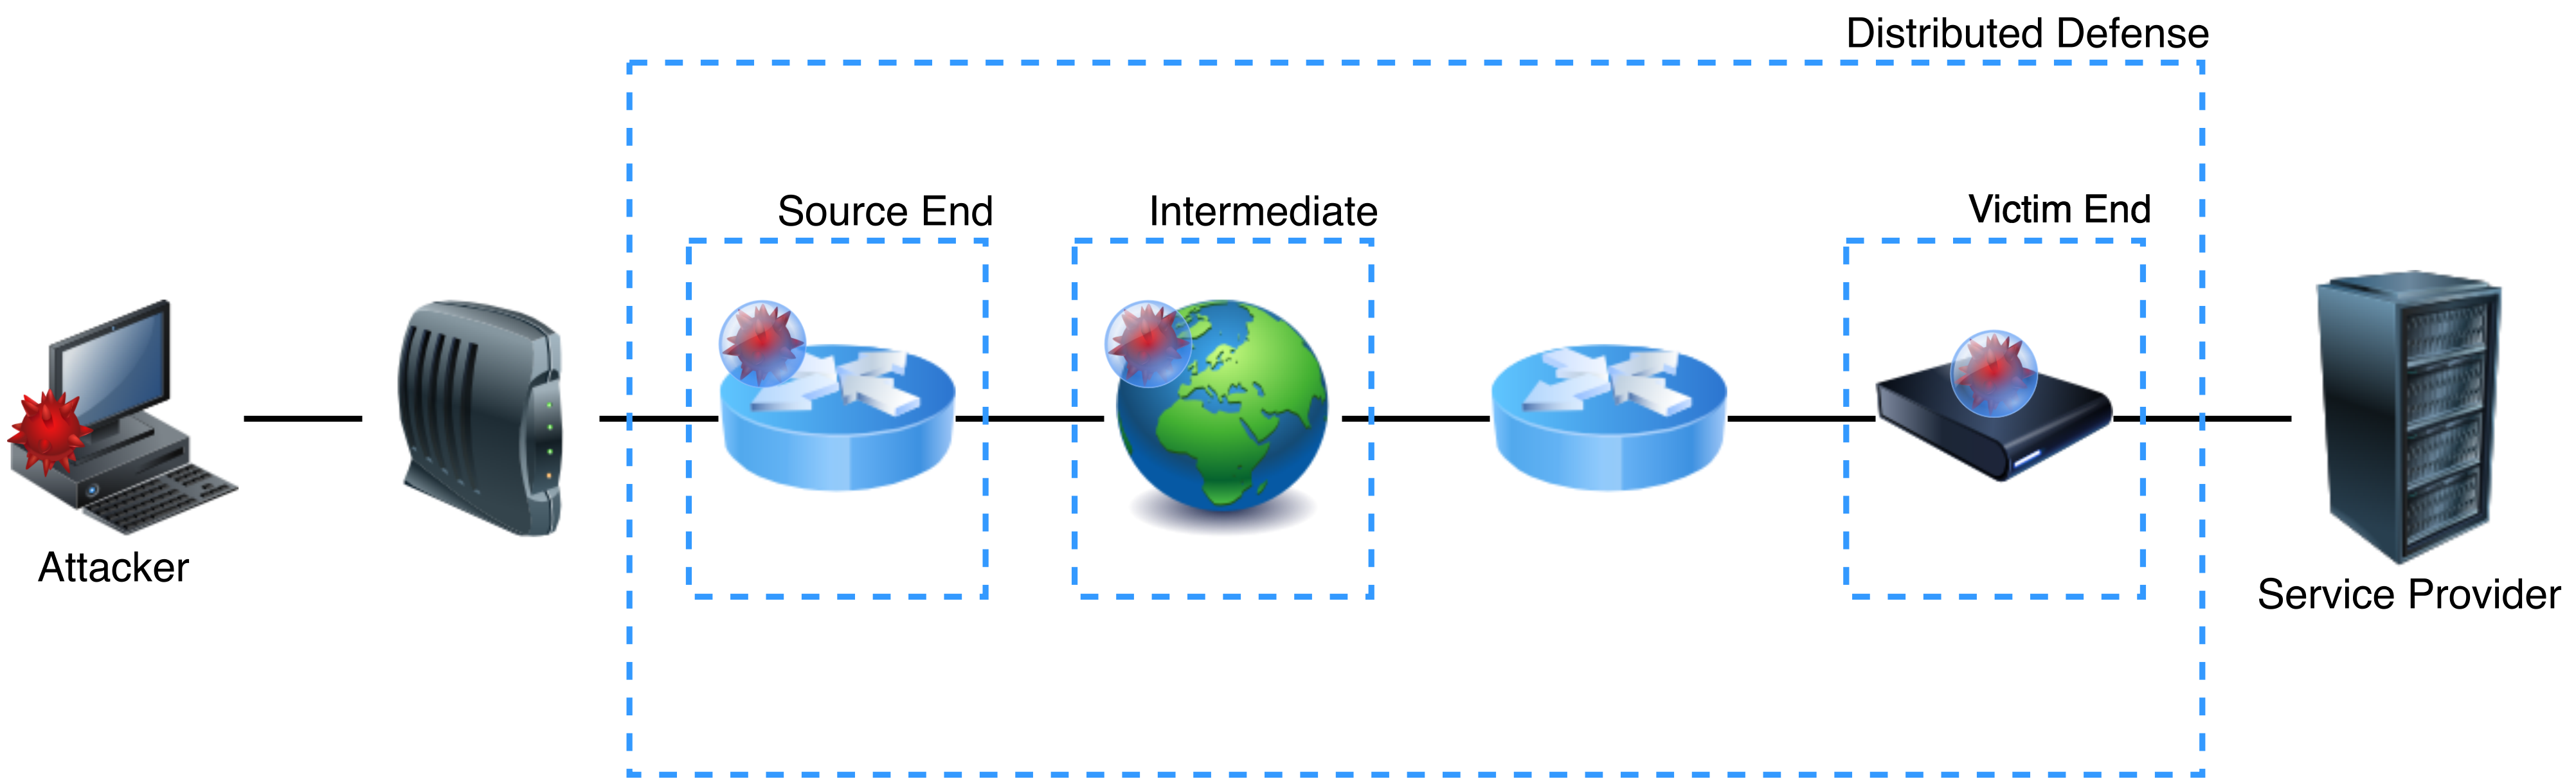
\includegraphics[width=3.5in]{locationOfDeployment}
\caption{Defense Deployment Location}
\label{fig_def}
\end{figure}

\noindent Other useful defense metrics are provided in Table \ref{tab:defMet}. 

{
\tabulinesep=1mm
\begin{table}[!htb]
  \centering
  \begin{tabu} to 0.5\textwidth {|X[1,r]|X[4]|}
     \hline
      Discrimination of Legitimate Traffic & In the traditional sense, there are two major principles of discriminating attack traffic between legitimate traffic: signature detection and anomaly based detection. Anomaly detection is dissected further into statistical (activity profiling) methodology, sequential change-point, wavelet analysis, and machine leaning \cite{Filtration:Kalkan}\\\hline
      
      Action Time Constraint & The defense mechanism is either \textit{proactive} or \textit{reactive}. This metric speaks to the time sensitivity of the solution in question, which can be critical to service providers depending on their needs.\\\hline
      
      False Positive Rate & Not only is it desirable to produce a system that will catch a multitude of DoS variants, it is also important to minimize interference with legitimate traffic. Because of this, a solution's false positive rate gives perspective on its effectiveness.\\\hline
      
      Scalability & It is desired that a solution be feasible both practically and financially to reach large scale deployments. On top of this, designs can be judged on their how modular they are; if they may be integrated with other defense systems easily.\\\hline
      
      Communication Overhead & In the case of a distributed system, the added requirement of communication between nodes deserves consideration.\\\hline
  \end{tabu}
  \smallskip
  \caption{Summary of Defense Metrics}
  \label{tab:defMet}
\end{table}
}

\section{Related Work}
Recent surveys in the area of DoS have been studied and considered in the crafting of this one. The work of Zargar \textit{et al.} provides a look into flooding-based DDoS defense mechanisms throughout the protocol stack and summarizes their advantages and shortcomings based on the location of network deployment \cite{Zargar:DDOSFlood}. Filtering,  D-WARD, reverse firewalls, IP traceback, and Management Information Base (MIB) are some of the topics covered in the network and transport layers. The final remarks of Zargar \textit{et al.}'s survey allude to potential future work in the area of DDoS prevention that is very much so being pursued today. A number of these points will be addressed in this survey.

A comprehensive insight into the inner workings of botnets and their role in elevating the devastation of DDoS attacks is presented by Hoque \textit{et al.} \cite{Botnet:Hoque}. This rigorous work outlines the different architectures of botnets down to their topology, administration, communication mechanisms, as well as issues challenges with their upkeep. The second half of the survey goes on to compare and contrast recent literature in the prevention of botnet based DDoS attacks through statistical methods, machine learning, and IP traceback. Hoque \textit{et al.} briefly relate their findings to paradigms such as cloud computing, big data analytics and SDN.

Kalkan \textit{et al.}'s survey on filtering based DDoS defense mechanisms diverges from the previous two in that their principle metric in classifying research is based on discrimination of traffic rather than network deployment location \cite{Filtration:Kalkan}. More specifically to filtration, this survey implements action time and collaborative properties to classify their findings. The contribution of Kalkan \textit{et al.} enumerates the available filtration techniques and addresses practical issues with a summary of each solution's deployment difficulty, communication overhead, scalability, and attack prevention efficiency. 

\section{Emerging Attacks}
\subsection{Flooding}
New flooding attacks are rather sparse, though not completely inexistent. One such attack turned up during this survey's literature review. It is called the Interest flooding attack \cite{Afanasyev:NDN}, presented by Afanasyev \textit{et al.}, and is specific to Named Data Networking (NDN).

In NDN, data is fetched by name using what are called Interest packets. These packets are routed to destination using the name and all intermediate routers keep a Pending Interest Table (PIT) with the necessary information to route the data back to the host that showed interest for it. This is what the Interest flooding attack takes advantage of.

In this setting, it is difficult for an attacker to target a specific host or router; however it is easy to target a namespace, say "\textit{/foo/bar}", that could very well be owned by a single data producer. The attacker then sends a high rate of Interest packets for this namespace (for names of the format "\textit{/foo/bar/...}"). This can cause a degradation of service in two ways: by creating network congestion, because Interest packets consume network capacity, and by exhausting resources on routers, since they need to maintain per-packet state for all forwarded Interest packets.

\subsection{Amplification}
Amplification allows attackers to significantly boost their throughput by coercing legitimate nodes into unknowingly taking part in an attack \cite{Krupp:Scan}. An amplification factor can be defined as a ratio of amplified traffic to source traffic. This also provides the attacker with a higher degree on anonymity since the traffic originates from elsewhere.

Literature review for this category turned up two different attacks, both presented in 2014 but remarkably absent from even the most recent surveys in the area.

The first one, The Greenhouse Effect attack \cite{GreenhouseEffect:Marchetta}, presented by Marchetta \textit{et al.}, allows the attacker to enlist unaware routers to hit its target with double the traffic that it sends. Accordingly, the attack has an amplification factor of 2.

To do so, it exploits a flaw in the Timestamp IP option and ICMP Parameter Problem scheme. This flaw, at the core, is that there is a limit to the number of timestamps that can be added to the packet, leading to an ICMP Parameter Problem error if reached \cite{GreenhouseEffect:Marchetta}. For the attack to work, it is also necessary that the victim replicates IP options from ICMP Echo Request packets into the Echo Reply packet it sends back.

The way it works is by first discovering the number of routers on the way to and back from the victim that support the IP Timestamp option. The simplest way to achieve this, though the authors also present a more reliable way to, is to send an Echo Reply packet with the IP Timestamp option to the victim, count the number of timestamps in the reply and assume half are on the way to the victim and the other half are on the way back. With this information, the attacker can then craft ICMP Echo Request packets by pre-filling with timestamps in such a way that the maximum number of timestamps will be reached when the Echo Reply packet goes through a router on the way back from the victim, meaning this router will send an ICMP Parameter problem packet back to the victim \cite{GreenhouseEffect:Marchetta}. This means the victim receives two packets for every packet the attackers sends and the resultant impact is performance degradation.

The authors, Marchetta \textit{et al.}, then conclude with statistics regarding the number of routers and hosts that are vulnerable to this attack. They found that 25.9\% of end hosts from Alexa's Top 5000 \footnote{http://www.alexa.com/topsites} are vulnerable and 34.3\% of routers from the iPlane project \footnote{http://iplane.cs.washington.edu/data/data.html} can be used as a reflector for this attack.

The second amplification attack that has been reviewed is the Store-and-Flood Distributed Reflective Denial of Service attack (SF-DRDoS) \cite{Liu:SFDRDoS}, presented by Liu \textit{et al.} This attack is specific to P2P networks such as Kad, which use a distributed hash table to store nodes' data on other nodes and make lookups over a connection-less protocol like UDP.

An attacker wanting to perform an SF-DRDoS attack will prepare by storing big chunks of data on multiple nodes in the network. Then, to start the flooding, it will spoof the victim's IP address and request all this data back. This result is all the store data being sent to the victim.

The authors claim an average amplification factor of 2400 in their experiments, with a peak at 4326. They also estimate that an attacker able to use all available nodes in the Kad network as reflectors could, with this average amplification factor and using only 280 Mbps, launch a 670 Gbps attack against a single victim, which is comparable to the largest DDoS recorded attacks \cite{Arbor:WISR}.\footnote{http://dyn.com/blog/dyn-analysis-summary-of-friday-october-21-attack/}

\subsection{Protocol-related Vulnerabilities}
The Low-rate DoS (LDoS), also known as the Shrew, attack preys on TCP's congestion control mechanism of Additive Increase, Multiplicative Decrease (AIMD) and the Re-transmission Timeout (RTO) \cite{Li:LAAEM}. The attack consists of three parameters: the attack rate, period, and duty cycle. They are chosen in such a way to trigger packet loss and, with the period of the attack corresponding to an integer multiple of the RTO counter, this may be done in a repetitively to severely reduce TCP's throughput. Variants of the attack which manipulate TCP's window of buffered packets have been proven to be quite effective as well \cite{Yue:shrew}. The impact of LDoS is degradation. For this attack, the rate need not be high (only large enough to cause some packet loss) which makes it hard to identify with traditional DoS defense systems \cite{Li:LAAEM}. Hence, the victim of such an attack is the link. An example of the LDoS attack of rate \textit{R}, period \textit{T}, and duty cycle \textit{D} is shown in Figure \ref{fig_ldosAttProf}:

\begin{figure}[!ht]
\centering
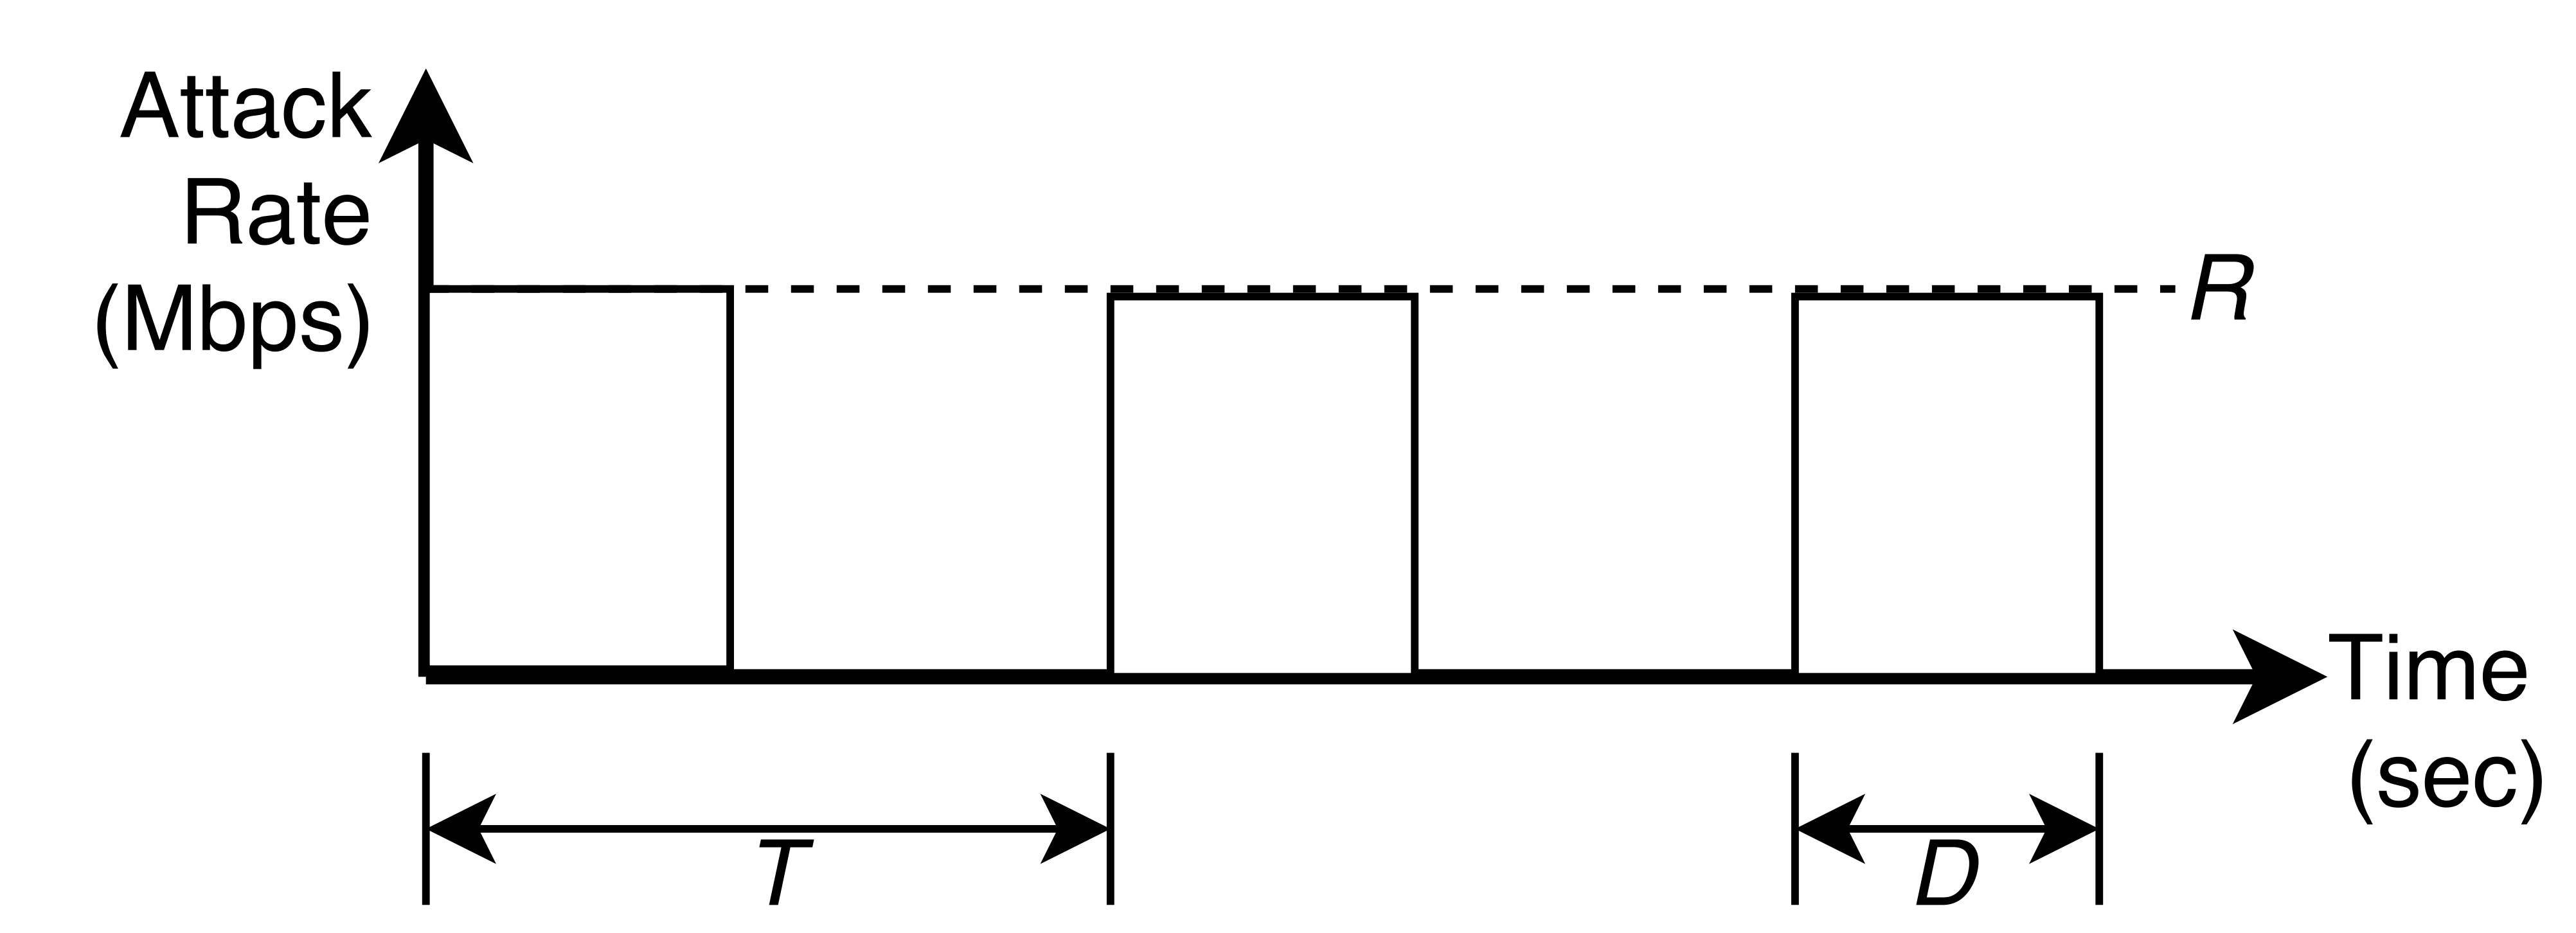
\includegraphics[width=3.5in]{LDoSAttProf}
\caption{LDoS Attack Profile with Duty Cycle \textit{D}}
\label{fig_ldosAttProf}
\end{figure}

While the LDoS attack is certainly not new, Li \textit{et al.} have proposed an infrastructure which seeks to enhance its abilities \cite{Li:LAAEM}. Their first observation is that this attack network may be scaled through use of a botnet. Next, Li \textit{et al.} note that the botnet's resources are not used efficiently due to the idle period of each zombie, as dictated by the nature of LDoS. Since many TCP connections use a recommended minimum RTO, it is assumed that the period parameter remains constant between connections. The authors take advantage of this characteristic and propose boosting the attack network's ability through slot multiplexing with multiple targets. An algorithm is presented by Li \textit{et al.} in order to achieve this goal.

An experiment carried out by these researchers consists of \textit{n} bots with uniform 1 Mbps link speeds are used to attack 100 targets. A random delay between bots and targets is used to more closely model a practical situation (delays need be taken into account with regards to each bots attack slot) where 5 different attack duty cycles are each simulated 100 times. It was found that, compared to the baseline of no multiplexing, the developed algorithm could reduce the number of bots needed, \textit{n}, by a factor of up to 9.02 to produce the same result \cite{Li:LAAEM}.

An RFC, 5961 \cite{Dalal:blindInWindow}, which seeks to improve TCP's robustness to blind in-window attacks may also be discussed in this category. Blind in-window attacks are those where a malicious user is able to discern a TCP connection's 4-tuple and inject data by providing sequence numbers in the permissible receive window at that instant. As explained by the RFC, the recent trend of applications making use of very long-lived connections, guessing the aforementioned parameters becomes less trivial. For this reason, extra security is proposed with a challenge ACK issued by the receiver as well as global rate limiting on TCP control packets. Linux systems have implemented this specification since kernel version 3.6's 2012 debut and it had also been backported to select releases \cite{OffPath:Cao}.

Cao \textit{et al.}, however, have uncovered a serious oversight in this specification which leads to a rather quick and reliable path to session hijacking as well as TCP RST injection DoS attacks \cite{OffPath:Cao}. The researchers cite the vulnerability as an aftereffect of changes in the way TCP connections are set up. A limit is imposed on the number of challenge ACKs generated per second - set to a default of 100. This however, is a global system variable which evidently implicitly leaks information to side channels allowing attackers to make inferences as to the existence of a connection with a specific 4-tuple and the next expected sequence and ACK numbers. Cao \textit{et al.} note that alternative off-path attack methodologies are not as capable due to their limitations in obtaining this information.

They go on to describe the practical implementation of RST injection DoS and session hijacking attacks based the security flaw introduced by this global resource. The attack network requires only a single agent, consists of a rather low rate (reset packets), and can cause outright denial of a victim to a service. Cao \textit{et al.} had found that, for their specific test environment, the RST DoS attack that was devised had an average success rate of 97\% and execution time of 44.3 seconds. In their work, these researchers have recommended phasing out this shared counter to eliminate the threat and have pledged to alleviate this issue in the Linux kernel. This framework had not been realized in Windows or Mac OS X, leaving them impervious to such exploits \cite{OffPath:Cao}.

\subsection{Packet Malformation}
In the area of packet malformation, this survey's literature review turned up no new research. That is, no outright new DoS attacks nor optimization to existing attacks relying on packet malformation were identified. Historic examples of malformed packet based DoS attacks include the Ping of Death (PoD) and the Local Area Network Denial (LAND) attacks \cite{SecuringCloudServers:Chapade}. 

\section{Emerging Defense Techniques}
\subsection{Source End}
Defense mechanisms deployed at the source network are rather uncommon in comparison to those deployed at other locations. Hence, this survey's literature review revealed no new such mechanisms. Less recent examples of source-based approaches include ingress/egress filtering at the source's edge routers, D-WARD, MUlti-Level Tree for Online Packet Statistics (MULTOPS) and MANAnet's reverse firewall \cite{Zargar:DDOSFlood}.

\subsection{Victim End}
Revisiting LDoS, two recent papers published by Wu \textit{et al.} \cite{Wu:LDoSMultifractal} and Bhuyan \textit{et al.} \cite{Bhuyan:partialRank} seek to provide a higher degree of detection, and ultimately mitigation, against such attacks. Both methods are deployed at the victim end and employ statistical methods to discriminate against attack traffic.

Wu \textit{et al.} present an analysis on the sensitivity of a statistical parameter, known as the singularity exponent, to LDoS attacks. The argument is that in a large scale, network traffic exhibits self-similarity while as a small-scale time series it is multifractal \cite{Wu:LDoSMultifractal}. The researchers look into the affect LDoS attack pulses have on the singularity exponent through a Multifractal Detrended Fluctuation Analysis (MF-DFA) algorithm. Next, the researchers present their developed algorithm in the estimation of the singularity exponent based on network traffic. Through their experimentation, it was found that as traffic becomes bursty, the singularity exponent decreases. In these tests, the ideal detection threshold was found as 0.6 --- offering a detection probability of 92\% along with a false positive and false negative rate of 9\% and 8\%, respectively \cite{Wu:LDoSMultifractal}.

Bhuyan \textit{et al.} estimates a parameter known as the correlation coefficient to determine the pairwise linear relationship of sampled network traffic. This value is bounded between [-1,1] signifying the amount of similarity --- with zero being none at all. They then calculate the partial rank correlation based on the already calculated correlation coefficient and this rank is compared to pre-defined thresholds. Two assumptions made in this work are that pairs of attack traffic have a rank of 1 and that attack and legitimate traffic follow Poisson and Gaussian distributions, respectively \cite{Bhuyan:partialRank}. That being said, the definition of such thresholds is highly dependent on an initial training phase containing both legitimate and attack traffic.

Although not particular to LDoS, the work of Tan \textit{et al.} also employs statistical correlation analysis to detect DoS attacks \cite{Tan:MCA}. Multivariate Correlation Analysis (MCA) is employed in order to address the issues of LDoS attacks that linearly change commonly monitored features to avoid detection as well as only being able to identify \textit{all} packets in a sample as either legitimate or not. This is accomplished by considering traffic samples individually. In addition, this method requires no historical traffic profiling to carry out analysis.

First, ingress traffic is monitored in order to build a network profile. Next, MCA is performed; Tan \textit{et al.} present an optimized algorithm employing a triangle area map scheme. This scheme identifies how the features of a sample series are geometrically correlated. Lastly, an anomaly based detection system is used in acting upon the features discovered by MCA. This system requires a 'normal profile' and a tolerance of deviation \cite{Tan:MCA}.

In benchmarking this solution, the researchers have put it up against six different DoS attacks. While the back, Smurf, and pod attacks were detected at rates in the high 90s (with a threshold of 3 standard deviations of the Mahalanobis Distances) whereas the teardrop and Neptune attacks were detected at a rate of about 50\%. The LAND attack was not detected at all. At the same threshold as above, the false positive rate was found to be 0.53\% \cite{Tan:MCA}. These deficiencies were addressed by Tan \textit{et al.} by use of data normalization which improved the detection rate of all the tested attacks at the cost of a larger false positive rate.  

Another form of victim end defense is an affirmation challenge which appears in the form of a puzzle. Such puzzles are intended to be easily generated by the server, reasonably difficult to solve for the client, and --- again --- easy for the server to check the answer's correctness. For instance, during a potential DoS attack originating form many different spoofed IP addresses; in this situation, the server will not expedite client requests or allocate memory until the correct solution is given. This mechanism can be prone to solution replay attacks by savvy clients.

With puzzles, there is no discrimination of legitimate traffic as all clients must bear the burden. This infrastructure is meant as a deterrent for attackers since establishing a connection to the content provider will waste their resources. For this reason, puzzles can be thought of as having a preventative action time. Also, it is noted by work in this area that dynamic puzzle difficulty based on the server's instantaneous workload has not been explored. Abliz \textit{et al.} introduce productive puzzles to address the issues of dynamism, solution replaying, and providing some utility out of the entire process. 

These so-called productive puzzles are a novel system for safeguarding against DDoS attacks \cite{Abliz:Puzz}. They intend to utilize undertakings from real applications and administrations rather than tedious cryptographic calculations for the sole purpose of posing a challenge to the client. With a generic puzzle generation framework, the output of the framework can be tailored to yield a solution relevant to a particular service. A Productive Puzzle Protocol (PPP) is presented by the authors to achieve these objectives. Moreover, a novel cache calculation is developed in consideration with the replay attack. Finally, Abliz \textit{et al.} assess the server's workload so that the difficulty is proportional. 

\subsection{Intermediate}
Miao \textit{et al.} present a real-time method for detecting Internet-wide SYN flooding attacks that can be deployed at network borders like Points of Presence (PoP) \cite{RealtimeDetection:Miao}. It works by first identifying eight attack scenarios based on whether the attacker is inside of a certain network $N$ or not (called the position of the attacker), the position of the victim and the position of the source IP address. Then, this method records metrics on SYN and SYN-ACK packet flow in five-minute intervals and, using an anomaly detection function on these metrics, builds a detection vector. Each attack scenario can then be mapped to a unique pair composed of the position of the victim and the detection vector using an algorithm the authors called WSAND.

This detection method has been implemented and used on 28 PoPs in the China Education and Research Network (CERNET) since the end of 2013. Attacks detected in March 2014, of which there were 207622, are discussed in the paper. The team behind this research manually validated part of those detection using (incomplete) IP traces and found that 92.5\% of them were correct, while the rest were either false positives or the IP traces didn't contain enough information for validation. The team plans on capturing complete packet traces to perform more thorough validation in the future.

On the other hand, Bohatei \cite{Bohatei:Fayaz} is a flexible and elastic DDoS defense presented by Fayaz \textit{et al.} that aims at neutralizing high-rate attacks provided that characteristics of the malicious traffic are known, from a detection mechanism like Miao \textit{et al.}'s discussed above, for example. While it could also be used at the victim's end, the authors see it as a better fit for Internet Service Providers to provide DDoS-protection as a service. Another objective of Bohatei is to require no expensive specialized hardware, but rather work on commodity hardware, reducing cost and increasing ease of deployment and scalability.

The idea of this approach is to redirect malicious traffic to defense Virtual Machines (VMs) that act as honeypots. The paper presents the Bohatei workflow as follows: first, the attack is detected by the Internet Service Provider (ISP) using an out-of-band anomaly detection technique and coarse specification of the malicious traffic is given. Then, Bohatei estimates the volume of malicious traffic --- that matching the given specification --- and allocates resources accordingly. This includes determining the type, number and location of defense VMs that need to be instanciated to minimize latency and network congestion, a task for which the researcher team has developed efficient algorithms. Finally, Bohatei makes use of SDN to set up forwarding rules to steer malicious traffic to the defense VMs.

\subsection{Distributed}
Implementing concepts from cloud computing and Content Delivery Networks (CDN), Wood \textit{et al.} present DoS Elusion (DoSE). The authors note that this solution is meant for medium sized service providers which would otherwise have little cost-effective options and is designed not to pose any new requirements to core networking infrastructure. Clients of a DoSE protected service are unknowing of the server's true location. Rather, they connect to an overlay network comprised of relay nodes. In this context, relays are cloud VMs which are loaded with forward firewall and filtering software \cite{Wood:DoSE}. Only clients assigned to the relay appear in the firewall's whitelist and rate limiting of each client is based on their track record. Elasticity of these relays is a critical feature provided by the cloud environment --- they can be quickly taken down during an attack and new relays may be spawned. This makes the solution fairly scalable.

Assignment of clients to relays utilize a secure push-based CDN system for the purpose of fast, client specific reassignment. The client must solve a puzzle whose answer is the name of a unique file hosted on a CDN, giving the details of the relay to which the client is assigned. This scheme keeps track of each client to whom a specific relay address is divulged. In the event that a relay is brought down, the associated clients may be deemed suspicious may be redistributed to lower priority nodes. For this reason, the action time constraint is reactive in that an attack must have occurred in order for further action to take place. In regards to identity concealment, all \textit{new} clients are initially deemed suspicious as well. When nodes are persistently taken down this method is theoretically able to isolate the client common to each attack \cite{Wood:DoSE}.

In a simulation with 1000 legitimate clients and one attacker connecting to the service all at once, the attacker is identified in 3.9 minutes while satisfying an average of 88.2\% of requests at that time \cite{Wood:DoSE}. The peak number of relays needed was 16. Other experiments conducted by Wood \textit{et al.} include multiple attackers as well as attackers present at the start-up of DoSE. Although attacks powerful enough to take down large data centers (cloud infrastructure) are not in the scope of this paper, the researchers boast a low-cost (under \$100/month) DoS elusion system for smaller service providers.


Another technique is IP traceback, which can be implemented to, in a sense, triangulate the origin of an attacks. The goal of IP traceback is to construct a path from source to destination for an IP packet even if it has been spoofed. This operation requires that forwarding devices along the way between source and destination be involved. IP traceback may be in the form of packet marking, logging, link testing, overlay, backscatter, or hybrid tracing according to Yao \textit{et al.} Each of these categories can even be further divided. With these methods, it is possible to combat the spoofing aspect of DDoS attacks. At the same time however, for the sake of deployment, it is desirable that these forwarding devices shouldn’t need any major rework or excessive memory consumption.

Of the above listed schemes, packet marking is quite popular in that its memory consumption is rather economical. During this procedure, forwarding devices inject a unique identifier into packets so to construct a path \cite{Yao:IPTraceback}. Probabilistic Packet Marking (PPM) and Deterministic Packet Marking are two different techniques. In PPM a node on the path injects its information into packets according to a probability distribution while DPM is on the basis of all ingress packets.

Unique Flow Marking (UFM) is proposed by Aghaei-Foroushani \textit{et al.} as an improvement to their novel work in the area of IP traceback. Previous implementations of their work, dubbed Deterministic Flow Marking (DFM), have embedded the source information of \textit{every} ingress flow to edge routers whereas UFM simply marks unique flows. This is done to reduce the number of required markings while still maintaining a high traceback rate. Flows are identified by their 5-tuple and 6-tuple for TCP/UDP and ICMP, respectively \cite{Aghaei:UFM}. Requiring many edge routers to support this, however, adds to the difficulty of deployment. 

The novelty in this solution is that it departs from the recent trend of PPM based techniques and is still quite efficient. Methods published in the realm of PPM, such as that of Nur \textit{et al.} \cite{Nur:CyPhy}, are economical on computing time but may require more complexity when a forward path needs to be reconstructed \cite{Aghaei:UFM}. Due to the nature of IP traceback itself, this solution's action time constraint is purely reactive.

The marking consists of the IP address of the router's egress interface and IDs assigned to the router's interface and origin MAC addresses, totaling 60 bits. A one bit flag is also used to identify marked packets. UFM encoders keep a table for accounting purposes. Similarly, UFM decoders are present at the destination end and use the marked data to infer the origin of the traffic, even if the IP is spoofed --- maintaining its own accounting table. Aghaei-Foroushani \textit{et al.}'s experimentation, in comparison to marking every packet (DPM), shows that UFM requires marking up to 95\% fewer packets and falls short at most by 6\% of successful tracebacks \cite{Aghaei:UFM}.

With DDoS attacks on the rise, there has been a big push to roll out distributed defense systems. One logistical issue this poses is the exchange of threat information between trusted sources. That being said there is no \textit{de facto} standard dictating such communications. This challenge is taken on by Steinberger \textit{et al.} through the use of Flow-based Event Exchange (FLEX) and Streaming Text Oriented Protocol (STOMP) \cite{Steinberger:FLEX}. STOMP is, as the authors put it, language-agnostic and of a publish and subscribe architecture whereas FLEX is used to structure the payload. These two underlying protocols are widely supported on different platforms --- ensuring scalability. 

Each collaborator is to provision a Mitigation and Response (MiR) system which handles events raised by partners. It is up to the ISP to decide on an MiR which is also responsible for distinguishing between legitimate and attack traffic. Upon processing events from the trusted partners, the goal is that each node will be able to create blocking policy on the fly.

In their experimentation, Steinberger \textit{et al.} simulate a SYN Flood originating within two different ISPs directed at another ISP. With attack traffic at a rate of 0.3 Gbps, lasting 42 seconds, it took 6 seconds and 18 messages for the 5 ISPs to come to an understanding and apply the appropriate policy to mitigate the attack.

\section{Interpretation and Discussion of Findings}

It was found that the attack classifications adopted from \cite{Botnet:Hoque,Zargar:DDOSFlood} are still relevant in regards to recent findings. That is, no new research in the field constitutes a brand new category. This does not come as a surprise due to the maturity of studies in DoS. Furthermore, it was found that most advances in DoS stem from either oversights in protocol specifications or operating under the assumption that a design will not be misused or abused (as seen in \cite{DoSTCPAnalysis:Schuba,Li:LAAEM,OffPath:Cao}). Attacks based purely on bandwidth exhaustion, flooding, and even malforming packets are not as active.

In the case of defenses, a wealth of information was revealed by the literature review of this survey. It is noted that purely source end solutions have not been as recently active as other categories. Observations explaining this are compiled in Table \ref{tab:defense}. The surveyed mechanisms expand on, and optimize, existing techniques and others make use of paradigms with growing popularity. Examples of this are found in the use of the cloud environment to provide cost-effective DoS Elusion and SDN as with Bohatei. As these systems become increasingly sophisticated and distributed, they must consider practicality. Such is covered in Steinberger \textit{et al.}'s efforts to standardize a collaborative event-based messaging protocol.

%TODO

{
\tabulinesep=1mm
\begin{table}[!htb]
  \centering
  \begin{tabu} to 0.5\textwidth {| X[1,r] || X[1,c] | X[1,c] | X[1,c] |}
     \hline
      & Deployment Difficulty & Communication Overhead & Action Time Constraint \\\hline\hline
     Source       & High   & Medium & Low    \\\hline
     Victim       & Low    & Low    & High   \\\hline
     Intermediate & Medium & Medium & Medium \\\hline
     Distributed  & Medium & High   & Medium \\\hline
  \end{tabu}
  \smallskip
  \caption{Comparison of Metrics by Network Deployment Location}
  \label{tab:defense}
\end{table}
}

\section{Conclusions}
In this paper, we briefly discussed DoS/DDoS attacks before presenting a classification and taxonomy inspired by previous surveys in the field for both attacks and defense mechanisms. We then introduced recent research papers on the subject of DoS attacks targeting the network and the transport layers, followed by defense techniques against such attacks, all of which we classified and characterized following our taxonomy. Finally, we interpreted and discussed our findings.

Though DoS is a very mature field and research in the area is abundant, it is still in evolution and problems still remain unsolved. Defense techniques are making great advances, becoming more and more effective and sophisticated as we have shown, but the effectiveness of even the most recent attacks such as the one targeting Dyn\footnote{http://dyn.com/blog/dyn-analysis-summary-of-friday-october-21-attack/} demonstrate that work still needs to be done in that regard.

\bibliographystyle{ieeetr}
\bibliography{papers.bib}
% use section* for acknowledgment
%\section*{Acknowledgment}
\end{document}